\section{Design}
In this section we designed the system architecture, and created various diagrams to explain how the different parts of the system work.


\subsection{Server-side}
The diagram shown on \ref{fig:serversidestructure} describes the overall structure of the server-side of the system. The server-side consists of both the Web-API and the control panel. These has been combined since they both interact with the same database and both has the same model. 

\begin{figure}[H]
    \centering
    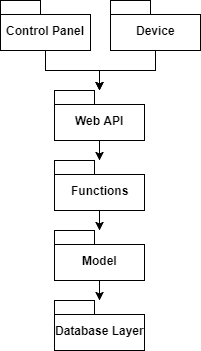
\includegraphics{Figures/serverSide.png}
    \caption{The structure of the server-side part of the system}
    \label{fig:serversidestructure}
\end{figure}

The function-layer is split into two parts, one for the control-panel and one for the API. This is done to isolate the functionality, such that each component only has access to their needed functionality. The shared model layer is described on \ref{fig:serversidemodel}.

\begin{figure}[H]
    \centering 
    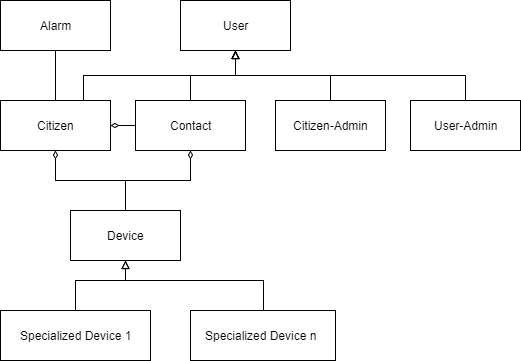
\includegraphics[width=0.9\textwidth]{Figures/serverSidemodel.png}
    \caption{The serverside model}
    \label{fig:serversidemodel}
\end{figure}

% The class-diagram on \ref{fig:serversidemodel} describes the model-layer, and the relations between the different parts of the model-layer.

\subsection{Web-Service}
When designing a web-service, it is important to consider which architecture to use and how to facilitate the communication to and from the service. Considering the requirements given in \ref{sec:non-requirements}, the architecture must allow for 
%we need a way to interact with it. Here we will look at different ways to interact with a server or service through the use of a Web-API.

\subsubsection{REST}
\todo{source pdf}
REST is based on the HTML protocol, and a REST system allows a client to communicate by using HTTP messages.
The four common message types used in REST are:

\paragraph{GET} gets a representation of a resource. The use of GET should never have side effects, and multiple calls to get should always give the same result.
\paragraph{DELETE} deletes a resource. Trying to delete a resource that doesn't exist usually results in an error response, such as 404. DELETE is also idempotent, so sending it multiple times does not cause any damage to the rest of the system, should it be sent twice.
\paragraph{POST} creates a new resource. Unlike DELETE, POST is not idempotent, so sending the same request twice will create the resource twice. 
The standard also allows POST to be overloaded. POST can do any change: DELETE, PUT, PATCH. When overloading POST, there are no protocol semantics it has to follow.
\paragraph{PUT} updates\todo{replace?} an existing resource. PUT is also idempotent, as sending the same PUT message multiple times will just update the resource to what it already is. Put can also work as POST for when the resource does not exist.


Another HTTP message is PATCH, which works as a partial put, where only some parts of a resource are updated.

REST also have six constrains that have to be fulfilled for the Web-API to be RETSful.

\paragraph{Uniform Interface}  There are four principle for a uniform interface:
\begin{itemize}
\item Resources are identified using URIs, and the data sent between the server and client are not the database, but an representation in HTML, XML or JSON.
\item The representation of data is enough to modify or delete it from the server.
\item The message contains information about how it should be parsed, and if it is cacheable.
\item Clients and server exchange resources in the form of hypermedia.
\end{itemize}
\paragraph{Stateless} A REST implementation is stateless if the server has no knowledge of the state of the client. All relevant data for the state of the client has to be sent to the server at each call, and nothing is kept between calls.
\paragraph{Cacheable} Some responses can be cached, while others cannot. So a resource must know if it can become stale between uses.
\paragraph{Client-Server} Clients should not be concerned with storage of data, while the server should not be concerned with user interface or user state. As long as the interface between server and client is unaltered, they can be developed independently.
\paragraph{Layered System} A client cannot tell if it is talking to the endpoint, or an intermediary. This allows load-balancing as multiple intermediary servers can run on multiple physical units, and still connect to the same end-point.
\paragraph{Code on Demand} The server can extend its functionality by sending logic that can be executed by the client. This step is unlike the others optional for an API to be RESTful.



\begin{comment}
\subsubsection{WSDL}
%https://www.w3.org/TR/wsdl
WSDL is an XML format that is used to describe network services as a set of endpoints, that each operate on messages containing document- or procedure-oriented information.

\subsubsection{SOAP}
\end{comment}

\subsection{Control panel}
The diagram shown on \ref{fig:controlpanel} describes the different views in the control panel. The login view is the view shown, when a user must login to the control panel.\\
The admin view, is the view shown to users with administration rights. The view will make the admin able to add new users to the system from the view.\\
The citizen view is for users with citizen-admin rights. The view will show the information on all the citizen the citizen-admin is administrating.

\begin{figure}[H]
    \centering
    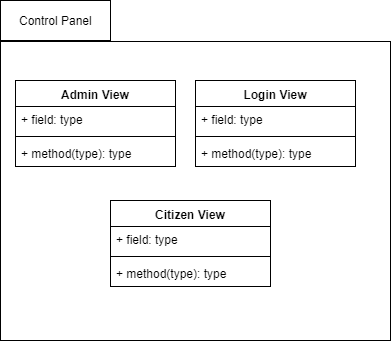
\includegraphics[width=0.5\textwidth]{Figures/ControlPanel.png}
    \caption{The different views included in the control-panel}
    \label{fig:controlpanel}
\end{figure}

\subsection{Smartphone app}
The android app is to show case the other aspect of the product, since the main focus of this project is not and smartphone app but on a IOT solution, this app is created with the bare minimum to be able to show case what our Rest-Api.

\begin{figure}[H]
    \centering
    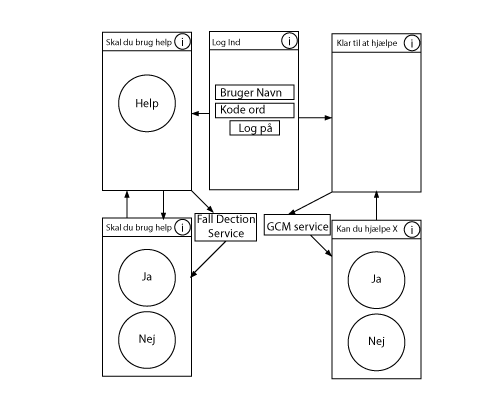
\includegraphics[width=0.7\textwidth]{Figures/MobilUI.png}
    \caption{Prototype of smartphone UI}
    \label{fig:mobilUI}
\end{figure}

In the figure \ref{fig:mobilUI} we have a over view of the app and the traversal through it, it start at the log in where it splits to left and right, the left side is for citizens that can call for help and start a background service to watch for a fall incident, and the right side is for contact persons this start a service to watch for Google cloud message. If the user say they need help or they can help citizen X then the app will contact the Rest-Api where it will handle contact the contact person to ask for help or say to the citizen that help on the way.
A service is a process that can run without the main app but still interact with it, example would be Facebook message app that alert you of new message even if you don't have it open or a music player that play the music even if the smartphone is in standby.

\subsection{Personal assistant}

\subsection{Communication}
